\apendice{Documentación técnica de programación}

%%INTRODUCCION
\section{Introducción}
En este anexo se describe la documentación técnica de programación para este proyecto. Incluye los primeros pasos que son la instalación del proyecto, la estructura de la aplicación o finalmente como compilarlo, desplegarlo o los diferentes tipos de configuraciones realizados. La idea es poder facilitar a los futuros desarrolladores una guía con la que poder comenzar, en el caso de que quisieran continuar con el trabajo.

%% eSTRUCTURA DE DIRECTORIOS
\section{Estructura de directorios}
El repositorio se encuentra alojado en \href{https://github.com/scc0034/flutter_serpiente}{Github}. La estructura de ficheros que sigue es la siguiente, destacando algunos de los más importantes:

\begin{itemize}
\item \textbf{./}
Directorio raíz del que cuelgan todas los demás ficheros. Este contiene uno de los archivos más importantes, que es es \emph{pubspec.yalm}. Este archivos se usa para hacer las importaciones de lós paquetes con las funcionalidades que queramos dar a nuestra aplicación.

\begin{itemize}
	\item \textbf{build}: Este directorio contiene todo lo relativo a las compilaciones, es decir, tanto como para hacer las pruebas en local de la aplicación , o crear los \emph{releases} que creamos oportunos. Además contiene todo lo relativo a las conexiones con Android Studio y Firebase, ya que necesita hacer las llamadas a este para lanzar los emuladores con la máquina virtual correspondiente. Dentro de esta estructura algunos de los ficheros más importantes son:
	\begin{itemize}
		\item \textbf{key.properties}: propeidades de la key, ya que esta nos permite desplegar la aplicación en la \emph{Play Store}. Es algo que no se tiene que perder ni modificar, ya que es de sumo valor. 
		\item \textbf{app/google-services.json}: fichero que descargamos desde Firebase, para que la aplicación tenga las conexiones con este \emph{Cloud service}, es decir, contienen las claves de conexión. En el caso de que tengamos que lanzar la app con otro de servicio de Firebase, podemos hacerlo cambiando este fichero.
		\imagen{techprog/google-services.jpg}{Google services}
		\item \textbf{app/build.gradle}: Fichero que contiene lo necesario para hacer las compilaciones, ya que como vemos tiene el SDK mínimo y máximo con el que trabaja (limitando el número de dispositivos que son compatibles),el número de versión, ya que cuando lo subamos a la \emph{Play Store}, es algo que debemos de revisar, ya que si no vamos a tener problemas de versionado. Además de los parámetros usados en la clave como podemos ver en la siguiente imagen.
		\imagen{techprog/app_build_gradle.jpg}{app/build.gradle}
		\item \textbf{app/key/keysnake.jks}: clave cifrada generada mediante el comando \ref{fig:commandkey}, esta no se puede perder, ya que sin ella es imposible desplegar la aplicación en la \emph{Play Store}.Es conveniente hacer alguna copia de seguridad en local.
		
		\begin{figure}[H]
			\centering
			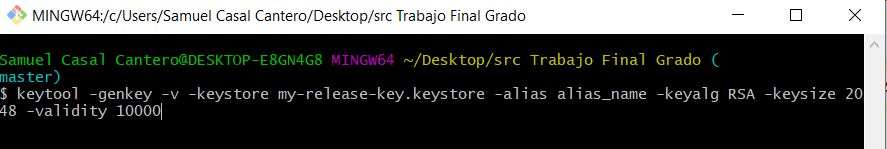
\includegraphics[width=1.0\textwidth]{/techprog/keysnakecommand}
			\caption{Comando generar clave keyStore}
			\label{fig:commandkey}
		\end{figure}	 
	\end{itemize}
	\item \textbf{assets}: directorio que contiene los activos de imágenes y audio de la aplicación. 
	\item \textbf{data/menu-opt.json}: fichero \emph{json} con la estructura del menú \emph{drawer}, con los nombres de ruta, nombre de icono y nombre de la página. 
	\item \textbf{docs/latex}: memoria y anexos del trabajo final de grado.
	\item \textbf{lib}: contiene los ficheros que se compilan para crear la aplicación. La estructura interna de directorios es la siguiente:
	\begin{itemize}
		\item \textbf{main.dart}: fichero principal del que cuelga toda la aplicación.
		\item \textbf{models}: contiene los modelos para crear las instancias de los objetos de la base de datos.
		\item \textbf{pages}: cada una de las interfaces o páginas de la aplicación.
		\item \textbf{providers}: proveedores de algunos servicios internos.
		\item \textbf{routes}: rutas de la aplicación.
		\item \textbf{services}: instancias a los servicios externos de la aplicación.
		\item \textbf{utils}: utilidades.
		\item \textbf{widgets}: elementos gráficos reutilizables.
		 
	\end{itemize}
\end{itemize}
\end{itemize}

%% MANUAL DEL PROGRAMADOR
\section{Manual del programador}
Este manual del programador tiene como objetivo ayudar a las personas futuras que estén interesadas en la continuación del proyecto, o simplemente que tengan ganas de aprender como se ha realizado. Para ello debemos de realizar las instalaciones de las siguientes herramientas:

\begin{itemize}
	\tightlist
	\item Flutter.
	\item Android Studio.
	\item Visual Studio Code.
	\item Git.
	\item Firebase Console.
	\item Play Store Console.
\end{itemize}

\subsection{Flutter:}
Es un SDK de código abierto creado por Google. Ofrece la versatilidad de crear aplicaciones móviles tanto como para \emph{iOS} y \emph{Android}, pero también para el entorno web. Internamente el lenguaje de programación es Dart.js, un \emph{framework}, que también es \emph{Open Source} desarrollado por Google, ya que pretende mejorar algunas de las carencias que tiene \emph{javascript}.

Para la instalación de Flutter debemos de ir a su \href{https://flutter.dev/docs/get-started/install}{web oficial} y descargarlo, dependiendo del sistema operativo que tengamos usaremos una versión u otra. (v.17.5 \emph{stable}).

Al descomprimir el fichero nos daremos cuenta de que tenemos un directorio (no ejecutables), por lo que debemos de dejar este en un lugar en concreto para después añadirlo a las variables de usuario. En mi caso yo lo deje en la siguiente ruta de mi ordenador personal C:$\backslash$src$\backslash$flutter.

Una vez tengamos el paso anterior debemos de actualizar las variables de usuario, apuntando al directorio bin de la ruta anterior, como vemos en la siguiente imagen:

\imagen{techprog/variablesEntorno.jpg}{Variables entorno}

Por defecto la rama de Flutter es la \emph{stable}, de las ramas disponibles: \emph{stable, beta, dev, master}. Pero si en el caso de necesitar la misma versión de Flutter, el comando necesario es:

\imagen{techprog/version}{Comando version Flutter}


\subsection{Android Studio:}
Es el IDE oficial de Google, que remplaza a Eclipse, basado en \emph{IntelliJ IDEA}, publicado de manera gratuita con Licencia Apache 2.0.

En nuestro caso, no programaremos en este IDE, ya que es complicado trabajar con Flutter directamente, solo lo vamos a utilizar para la creación de las máquinas virtuales para emular el sistema operativo Android. Por lo que descargamos de la \href{https://developer.android.com/studio}{web oficial Android Studio} e instalamos, en mi caso uso la versión 3.6.

Una vez lo tengamos instalado creamos las máquinas virtuales, para ello nos vamos a la barra de herramientas Tools>AVD manager y creamos las que sean necesarias, en mi caso tengo dos, con Andorid R, que es la versión 10 de sistema operativo, ya que es la última estable que nos ofrece el IDE.
\imagen{techprog/vm.jpg}{Máquinas virtuales}

\subsection{Visual Studio Code:}
Es el editor de código creado por Microsoft, permite mucha versatilidad y es eficiente para la edición del código en flutter. Es de código abierto bajo la licencia MIT.

Lo podemos descargar de la \href{https://code.visualstudio.com/}{web VS Code}, en mi caso uso la versión 1.47.

Una vez lo tengamos instalado, procedemos a instalar los siguiente \emph{Snippets} que nos ayudan a la creación del código, ya que son como los atajos de teclado. En cada uno de los enlaces, podemos ver una descripción de que es lo que hace cada una de estas herramientas:

\begin{itemize}
	\tightlist
	\item \href{https://marketplace.visualstudio.com/items?itemName=Nash.awesome-flutter-snippets}{Awesome Flutter Snippets}. Apache 2.0.
	\item \href{https://marketplace.visualstudio.com/items?itemName=CoenraadS.bracket-pair-colorizer-2}{Bracket Pair Colorizer 2}. MIT License.
	\item \href{https://marketplace.visualstudio.com/items?itemName=Dart-Code.dart-code}{Dart}. MIT License.
	\item \href{https://marketplace.visualstudio.com/items?itemName=Dart-Code.flutter}{Flutter}. MIT License.
\end{itemize}

\subsection{Git:}
Es un software para el control de las versiones, que nos permite trabajar mediante comandos desde \emph{Git Bash}, la licencia es GNU-GPL v2.  La última versión estable con la que he trabajado es 2.27 y la podemos encontrar \href{https://git-scm.com/}{web ofical}.

\subsection{Firebase Console:}
La consola de \href{https://console.firebase.google.com/?hl=es}{Firebase} es la que nos permite el control de todas las características de \emph{Cloud Services}, desde la autentificación de los usuarios, base de datos o AdMob services, entre otras muchas.

Al estar registrado con mi cuenta personal, os tengo que dar permisos de administrador en el caso de que fuera necesario, para ello no dudéis en mandarme un correo \href{mailto:casalyepa@gmail.com}{casalyepa@gmail.com}

\imagen{techprog/firebase.jpg}{Firebase console}

\subsection{Play Store Console:}
La consola de \href{https://play.google.com/apps/publish/?account=9184458375980004308#AppListPlace}{Play Store} es la herramienta web que nos permite hacer el despligue de la aplicación, tanto como para hacer las pruebas beta, o para subirla y que todo el mundo se la pueda descargar.

La revisión de cada una de las nuevas versiones puede tardar en ser validada, por lo que tenemos que tener paciencia.

Al igual que con Firebase, os tengo que dar permisos en el caso de que sea necesario hacer nuevos despliegues de la app \href{mailto:casalyepa@gmail.com}{casalyepa@gmail.com}

\imagen{techprog/playstore.jpg}{Play Store console}

%% 	COMPILACIÓN DEL PROYECTO INSTALACIÓN Y EJECUCION
\section{Compilación, instalación y ejecución del proyecto}
En este apartado se muestran los pasos necesarios para hacer una copia del proyecto en Github y poder trabajar en local desplegando la aplicación en los emuladores.

\subsection{Clonación del proyecto:}
\begin{enumerate}
	\item Nos colocamos en el directorio donde queramos tener el proyecto y abrimos \emph{git bash} mediante el botón derecho:\imagen{techprog/clonar.png}{Abrir git bash}
	\item Procedemos a clonar el proyecto con el comando : 
	\texttt{git clone \\https://github.com/scc0034/flutter\_serpiente.git}~\ref{fig:git-clone}
\end{enumerate}
\begin{figure}[H]
	\centering
	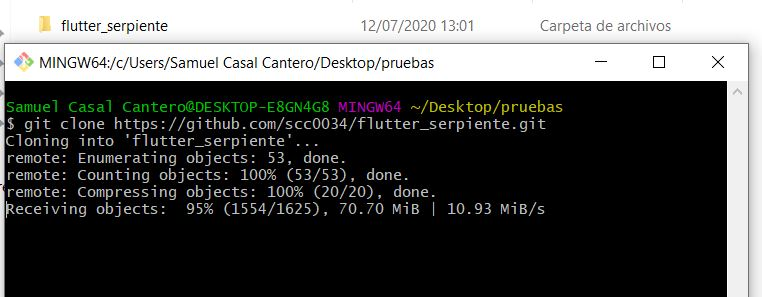
\includegraphics[width=1\textwidth]{techprog/gitclone.jpg}
	\caption{Comando para clonar el repositorio.}\label{fig:git-clone}
\end{figure}
\subsection{Instalación de los paquetes:}
Una vez tengamos el proyecto clonado, debemos de ejecutar el comando \texttt{flutter upgrade}, para traer todos los paquetes, ya que si no las importaciones de cada uno de las páginas van a aparecer como erróneas.

\begin{figure}[H]
	\centering
	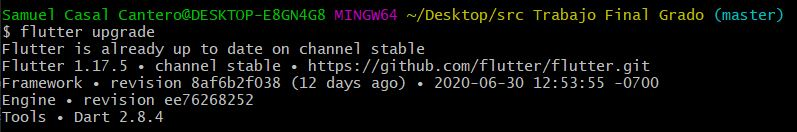
\includegraphics[width=1\textwidth]{techprog/flutterupgrade.jpg}
	\caption{Actualización paquetes}\label{fig:upgrade}
\end{figure}

Una vez lo hagamos debemos de reiniciar Visual Studio Code.
\section{Pruebas del sistema}
